\documentclass[coverpage,lineno]{../custom}
\usepackage[dvipsnames,table]{xcolor}
\usepackage{tabularx}
\usepackage{multicol}
\usepackage{multirow}
\usepackage{makecell}
\usepackage{pdflscape}
\usepackage{pgfgantt}
\usepackage{tikz}
\usepackage{ctable}
\usepackage{listings}
\usepackage{enumitem}
\usepackage[style=numeric-comp,alldates=iso,sorting=none]{biblatex}
\usetikzlibrary{arrows.meta}
\renewcommand{\cellalign}{lc}
\newcolumntype{L}[1]{>{\hsize=#1\hsize\raggedright\arraybackslash}X}
\newcolumntype{C}[1]{>{\hsize=#1\hsize\arraybackslash}X}
\newcolumntype{R}[1]{>{\hsize=#1\hsize\raggedleft\arraybackslash}X}
\definecolor{RedOrange}{RGB}{255,83,0}

\addbibresource{../references.bib}

\newcommand{\musthave}{{\color{red}Must have}}
\newcommand{\shouldhave}{{\color{orange}Should have}}
\newcommand{\couldhave}{{\color{Green}Could have}}
\usepackage{longtable}
\usepackage{boldline}
\usepackage{everypage}

\newcommand{\FunctionalReq}[8]{
\begin{longtable}{|p{0.225\textwidth}|p{0.725\textwidth}|}
\hline
	\textbf{ID - Name} & \textbf{#1 - #2} \\\hlineB{2}
	\textbf{Description} & #3 \\\hline
	\textbf{\makecell*{Priority - {\color{red}Mu\color{orange}Sh\color{Green}Co}}} & #4
	
	#5 \\\hline
	\textbf{Dependencies} & #6 \\\hline
	\textbf{Expected Results} & #7 \\\hline
	\textbf{Exception handling} & #8 \\\hline
\end{longtable}
}
\newcommand{\NonFunctionalReq}[7]{
\begin{longtable}{|p{0.155\textwidth}|p{0.795\textwidth}|}
	\hline
	\textbf{ID - Name} & \textbf{#1 - #2} \\\hlineB{2}
	\textbf{Type} & #3 \\\hline
	\textbf{Priority} & #4 \\\hline
	\textbf{Description} & #5 \\\hline
	\textbf{Metrics} & #6 \\\hline
	\textbf{Constraints} & #7 \\\hline
\end{longtable}

}
\newcommand{\NonFunctionalReqSec}[8]{
\begin{longtable}{|p{0.155\textwidth}|p{0.795\textwidth}|}
	\hline
	\textbf{ID - Name} & \textbf{#1 - #2} \\\hlineB{2}
	\textbf{Type} & #3 \\\hline
	\textbf{Priority} & #4 \\\hline
	\textbf{Description} & #5 \\\hline
	\textbf{Metrics} & #6 \\\hline
	\textbf{Constraints} & #7 \\\hline
\end{longtable}
}
\newcommand{\Risk}[4]{
\begin{longtable}{|p{0.125\textwidth}|p{0.825\textwidth}|}
	\hline
	\textbf{ID - Risk} & \textbf{\makecell*{#1 - #2}} \\\hlineB{2}
	\textbf{Risk} & #3 \\\hline
	\textbf{Mitigation} & #4 \\\hline
\end{longtable}
}
\newcommand{\RiskMatrix}[9]{
\begin{tabularx}{\textwidth}{C{0.15}C{0.65}|L{1.4}|L{1.4}|L{1.4}|}
	\cline{3-5}
	& & \multicolumn{3}{c|}{\textbf{Impact}} \\\cline{3-5}
	& & \makecell*{Low} & \makecell*{Medium} & \makecell*{High}\\\hline
	\multicolumn{1}{|c}{\multirow{3}{*}{\rotatebox[origin=c]{90}{\textbf{Probability }}}} & \multicolumn{1}{|l|}{Unlikely} & \cellcolor{Green}\makecell*{#1} & \cellcolor{LimeGreen}\makecell*{#2} & \cellcolor{YellowOrange}\makecell*{#3} \\\cline{2-5}
	\multicolumn{1}{|c}{} & \multicolumn{1}{|l|}{Possible} & \cellcolor{LimeGreen}\makecell*{#4} & \cellcolor{YellowOrange}\makecell*{#5} & \cellcolor{RedOrange}\makecell*{#6} \\\cline{2-5}
	\multicolumn{1}{|c}{} & \multicolumn{1}{|l|}{Likely} & \cellcolor{YellowOrange}\makecell*{#7} & \cellcolor{RedOrange}\makecell*{#8} & \cellcolor{Red}\makecell*{#9} \\\hline
\end{tabularx}

}

\newcommand{\Lpagenumber}{\ifdim\textwidth=\linewidth\else\bgroup
  \dimendef\margin=0 %use \margin instead of \dimen0
  \ifodd\value{page}\margin=\oddsidemargin
  \else\margin=\evensidemargin
  \fi
  \raisebox{\dimexpr -\topmargin-\headheight-\headsep-0.5\linewidth}[0pt][0pt]{%
    \rlap{\hspace{\dimexpr \margin+\textheight+\footskip}%
    \llap{\rotatebox{90}{\thepage}}}}%
\egroup\fi}
\AddEverypageHook{\Lpagenumber}%

\Title{Requirement Specification}

\begin{document}
\pagenumbering{gobble}
\maketitle
\tableofcontents\newpage
\pagenumbering{arabic}


\section{Introduction}
\label{sec:intro}

\subsection{Overview and Justification}
\label{ssec:just}

This document provides the requirement specifications for our virtual reality (VR) meditation application, referred to henceforth as `the product'; the specific software for the product shall be referred to as `the software'. This document provides an introduction (\cref{sec:intro}) to the project, covering the justification (\cref{ssec:just}), scope (\cref{ssec:scope}), and systems (\cref{ssec:desc}); the requirements for the system (\cref{sec:req}), both functional (\cref{ssec:f_req}) and non-functional (\cref{ssec:nf_req}), and potential risks and issues (\cref{ssec:risks}); the development of the project (\cref{sec:dev}) in terms of the approach (\cref{ssec:dev_approach}) and schedule (\cref{ssec:schedule}).

This project is for Professor Alexandra Cristea who shall henceforth be referred to as 'the client'. The client has given us the project of developing a VR meditation application with the possible use as a basis for research into the topic. This project aims to help those who have not done any, or have done very little, meditation before by giving them an immersive VR world to aid concentration and relaxation.

\subsection{Project Scope}
\label{ssec:scope}

This project is intended for those who have never done any, or done very little, meditation before. It is aimed primarily at adults. The app is intended to help with mindfulness meditation (MM) practice through the use of gamification concepts and VR. The primary objectives are as follows:

\begin{itemize}
	\item Personalisation over customisation\\
	The client would prefer for the project to personalise, that is automatic adjustments to suit the user, itself rather than have the user customise the project, that is allowing the user to alter the environment
	\item Stability\\
	The client would prefer fewer stable features over more less-stable features
	\item Modularity\\
	The client would prefer the software to be modular to allow for ease of reuse in future projects
\end{itemize}

The client would also like the potential to use the project later on in a research context. This is not a primary consideration of ours, but we will use this to guide our development. To ensure that our project can be as seamlessly used in this context with little impact on the project itself, we will make reference to relevant literature where necessary to ensure our implementations of MM is as concurrent with current literature as we can make it\footnote{The authors can find little research on MM with VR implementations. There is a significant amounts of research into VR applications and MM separately which we will use to guide our development}.

For some examples of literature we will likely make reference of, see \cite{kosunen_relaworld_2016, tang_neuroscience_2015, wang_reducing_2022}. We will also make significant reference to \cite{lan_slow_2021} as a good example of research into a similar topic.

\subsection{System Description}
\label{ssec:desc}

The system will be a VR app intended for meditation with aspects of gamification\cite{toda_taxonomy_2019} using the Meta Quest\footnote{Previously Oculus Quest}. The app is intended to aid with visualisation based meditation and to accelerate the progression through meditation training.

The primary section of the app will be set in an environment designed to have as little distraction as possible whilst still allowing the app to be engaging. At present, we intend for the environment to be relatively featureless, with some objects orbiting the user. The objects will themselves have particles around them to obfuscate any highly contrasting areas. Each session will be approximately 10 to 20 minutes in length and various metrics will be measured throughout such as heart rate, EEG data, and eye tracking. This will be analysed and stored externally in accordance with the GDPR.

Evaluation metrics will be applied to the raw data, the results of which will be used to compare sessions and measure improvement. These metrics will be user-specific and will require user-specific baseline data, as well as general data. To gather this baseline data, a short (at most 5 minutes) baseline session will be required before the user can complete any meditation.

The data metrics will be constructed to account for global limits and will be personalised, via user-specific data, to ensure that any change can be measured relatively to the user and not to some global standard. With this we aim to ensure that all users can see a clear progression from session to session.

Each user will have an associated account that will communicate with the server. This account will contain the user's name and personalisation data. The user will be able to access a history of sessions via a request to the server.

The server itself will be run by a Python script that can be run on any computer. For the purpose of product demonstration, we will ensure the same computer runs both the server and Quest app in lieu of a server with a static IP. The server will store user account data, raw session data, and session metric results. Data will be stored in a XML format, with each user having a folder under their username, with sessions and user data within that folder. Current, incomplete, XML DTD are given in \cref{apdx:xml_dtd}.

\subsubsection{Current systems}

There exists several current systems for integrating VR into meditation. We will briefly discuss two of these such systems here.

Lan et al. \cite{lan_slow_2021} demonstrated a feasible study for multimodal feedback meditation in VR. They used g-tummo meditation which has some well researched benefits \cite{kozhevnikov_neurocognitive_2013} but is a fairly advanced technique. As such the multimodal feedback system allows less experienced meditators to feel a more immediate feedback from meditation and thus attempt to help motivate people to continue meditation. This research showed that the multimodal feedback correlated with a decrease in breathing rate and helped maintain user attention, measured via tiredness.

Hølledig et al. \cite{holledig_zenvr_2018} demonstrated a VR based meditation environment also using biofeedback. Their environment was a generated forest environment with different amounts of fog depending on real-time evaluation of the user's meditative state. Whilst they failed to show any meaningful benefits, they do note that the use of biofeedback has potential to be useful. The authors also note of significant issue with the Myndplay headband that resulted in having to redesign their tests.

\newpage
\section{Solution Requirements}
\label{sec:req}

\subsection{Functional Requirements}
\label{ssec:f_req}

The functional requirements of our system can be broken down into three main types which are explained below:

\begin{description}[font=\bfseries, leftmargin=1cm, style=nextline]
\item[Sensor]
For the app to be adaptive, we need data coming in that will inform us of the user’s physiological state. To achieve this, we need to be reading data from sensors fitted on the user and passing it into our system. The proper functioning of such sensors through them being correctly fitted, configured, and consistently and reliably transferring data is what is meant by the sensor requirements.
\item[Environmental]
To utilise the advantages that VR has, when compared to more conventional types of meditation, we shall build an environment that the user can become immersed within. This will be achieved by designing the visual and audio elements to be coherent with one another. Such an environment should immerse the user not just through its design but through it adapting based upon the user’s physiological state. When referring to environmental requirements, this encompasses the design of the environment, whether that is the menus, the walkthrough, or the meditation, and how that environment adapts to sensory data.
\item[Data Collection]
Because of our app's potential to feed into research, it is important for the data not only to be used live to adapt the environment, but for it to also be stored for further analysis. When speaking with the client, the importance of data storage was made very clear to us, as she commented in our meeting that `if you remember anything from all of this, generate data from the people and from the environment and their interactions'.
We have thus designated all objectives related to the collection, storage, and processing of data underneath the data collection requirement heading.
\end{description}

\begin{figure}[t!]
	\centering
	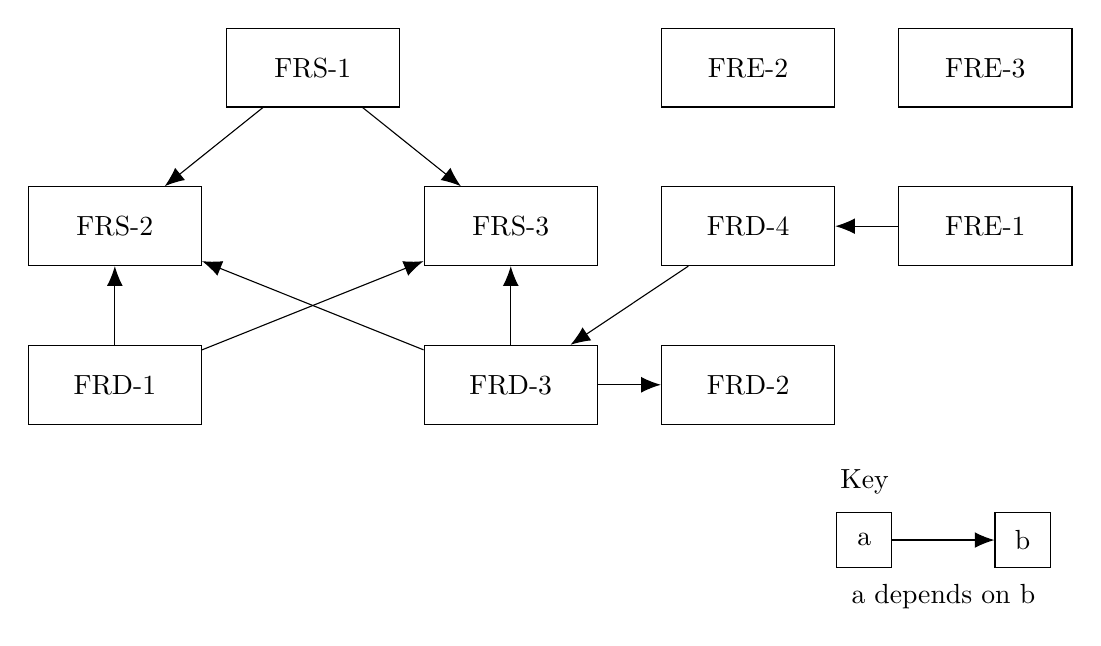
\begin{tikzpicture}[
		node distance=1cm and 0.3cm,
		auto,
		node/.style={rectangle, draw=black, minimum width=22mm, minimum height=10mm},
		keynode/.style={rectangle, draw=black, minimum width=7mm, minimum height=7mm}
	]
		\node[node](frs-1){FRS-1};
		\node[node](frs-2)[below left =of frs-1]{FRS-2};
		\node[node](frs-3)[below right =of frs-1]{FRS-3};
		\node[node](frd-1)[below =of frs-2]{FRD-1};
		\node[node](frd-3)[below =of frs-3]{FRD-3};
		\node[node](frd-2)[right =of frd-3,xshift=0.5cm]{FRD-2};
		\node[node](frd-4)[right =of frs-3,xshift=0.5cm]{FRD-4};
		\node[node](fre-1)[right =of frd-4,xshift=0.5cm]{FRE-1};
		\node[node](fre-2)[above =of frd-4]{FRE-2};
		\node[node](fre-3)[right =of fre-2,xshift=0.5cm]{FRE-3};
		
		\draw[-{Latex[length=2.5mm,width=2mm]}](frs-1) -- (frs-2);
		\draw[-{Latex[length=2.5mm,width=2mm]}](frs-1) -- (frs-3);
		\draw[-{Latex[length=2.5mm,width=2mm]}](frd-1) -- (frs-2);
		\draw[-{Latex[length=2.5mm,width=2mm]}](frd-1) -- (frs-3);
		\draw[-{Latex[length=2.5mm,width=2mm]}](frd-3) -- (frs-2);
		\draw[-{Latex[length=2.5mm,width=2mm]}](frd-3) -- (frs-3);
		\draw[-{Latex[length=2.5mm,width=2mm]}](frd-3) -- (frd-2);
		\draw[-{Latex[length=2.5mm,width=2mm]}](frd-4) -- (frd-3);
		\draw[-{Latex[length=2.5mm,width=2mm]}](fre-1) -- (frd-4);
		
		% key
		\node[keynode] at (7,-6)(a){a};
		\node[keynode](b)[right =of a,xshift=1cm]{b};
		\draw[-{Latex[length=2.5mm,width=2mm]}](a) -- (b) node[label={[yshift=9mm,xshift=-10mm]Key},midway,yshift=-1cm] {a depends on b};
	\end{tikzpicture}
	\caption{Functional dependency graph}
\end{figure}
The functional requirements of our system can be broken down into three main types: \textbf{Sensor, Environmental} and\textbf{ Data Collection}
 
For our meditation app to be adaptive, we need data coming in that will inform us of the user’s physiological state. To achieve this, we need to be reading data from sensors fitted on the user and passing it into our system. The proper functioning of such sensors through them being correctly fitted, configured, and consistently and reliably transferring data is what is meant by the \textbf{sensor} requirements.
 
To utilise the advantages that VR has, when compared to more conventional types of meditation, we shall build an environment that the user can become immersed within. This will be achieved by designing the visual and audio elements to be coherent with one another. Such an environment should immerse the user not just through its design but through it adapting based upon the user’s physiological state. When referring to \textbf{environmental} requirements, this encompasses the design of the environment, whether that is the menus, the walkthrough, or the meditation, and how that environment adapts to sensory data.
 
Because of our app's potential to feed into research, it is important for the data not only to be used live to adapt the environment, but for it to also be stored for further analysis. When speaking with the client, the importance of data storage was made very clear to us, as she commented in our meeting that “if you remember anything from all of this, generate data from the people and from the environment and their interactions”. 
 
We have thus designated all objectives related to the collection, storage, and processing of data underneath the \textbf{data collection} requirement heading.
\subsubsection{Sensor Requirements}

\FunctionalReq
{FRS-1}{Baseline Readings}
{Baseline readings should be taken for each new user of the software. This should occur over 90 seconds where the user remains seated without  the VR headset on}
{Medium - \shouldhave}
{Baseline values could be inferred from averages i.e. average heart rate for someone the same age, however, this wouldn’t be ideal}
{FRS-2, FRS-3}
{Obtain an average value for the heart rate, concentration and meditation values of the user prior to meditating.}
{If calibration fails then check the positioning of the sensors on the user and reposition if necessary. If that fails try again after resetting and restarting the failing sensor}

\FunctionalReq
{FRS-2}{Heart Rate Monitor Connectivity}
{The heart rate monitor should return readings at regular intervals through a Bluetooth connection}
{High - \musthave}
{For the application to be adaptive, it needs to have a constant data stream of heart rate data}
{None}
{Obtain a constant stream of data detailing the heart rate of the user at specific times}
{If calibration fails then check the positioning of the sensor on the user and reposition if necessary. If that fails try again after resetting and restarting the heart rate monitor}

\FunctionalReq
{FRS-3}{EEG Connectivity}
{The EEG should return readings at regular intervals through a Bluetooth connection}
{High - \musthave}
{For the application to be adaptive, it needs to have a constant data stream of values from the EEG}
{None}
{Obtain a constant stream of data detailing the concentration and meditation score of the user at specific times}
{If calibration fails then check the positioning of the sensor on the user and reposition if necessary. If that fails try again after resetting and restarting the EEG}

\subsubsection{Data Collection Requirements}

\FunctionalReq
{FRD-1}{Storing Sensor Data}
{EEG and Heart Rate readings should be stored with timestamps throughout the session}
{High - \musthave}
{As emphasised by our client, making sure to generate data that can be studied is perhaps the most important requirement of our system}
{FRS2, FRS3}
{Obtain an XML file for each session with EEG and heart rate data fields included}
{Identify whether the exception occurs because of the connectivity of the sensors or the code for producing data files. If it is the former case, then refer to exception handling for FRS2 and FRS3. If it is the latter case then not much can be done apart from providing a form for feedback as this would be a bug in the code}

\FunctionalReq
{FRD-2}{Storing User Behaviour}
{Behaviour about how the user interacts with the virtual environment should be stored with timestamps. This includes what their attention is focussed on and their movement}
{High - \shouldhave}
{Although generating data that can be studied is very important for our application, data that is collected from the sensors is of greater importance. Collecting data from how the user interacts with the environment could be difficult and so although we would like this to be done, it is not a must have requirement}
{None}
{Obtain an XML file for each session with user gaze tracking data}
{An exception occurring would mean a failure of the code. Not much can be done apart from providing a form for feedback as this would be a bug in the code}

\FunctionalReq
{FRD-3}{Performance of meditation is measured and displayed at the end of a session}
{The user's performance throughout the meditation exercise should be evaluated, and then displayed to them at the end of a session}
{Medium - \couldhave}
{Seeing how you performed after a session gamifies the program and gives the user insight into how well they have performed, but it is not a crucial feature from speaking to the client}
{FRS2, FRS3, FRD2}
{A value, calculated from a mixture of variables, including heart rate, meditation value (from the EEG), head movement. This value would indicate how well the user meditated}
{Two main types of exception could occur for this requirement. If the value is not well computed, i.e the formula used does not accurately indicate how well the user has meditated, a feedback form could be provided where users could share their opinion. The formula could be perhaps reworked in this case.

If some code means that the value calculated is not displayed or produces a value outside of the range of 1 to 100 then this is an error in the code. Not much can be done apart from providing a form for feedback}

\FunctionalReq
{FRD-4}{Past meditations performance is stored and can be displayed against session number in a graph}
{For a particular user, performance from session to session will be stored and can be displayed in a graph for them against the session number}
{Medium - \couldhave}
{Gamifying the meditation would help users become more motivated to continue as they would  tangibly be able to see their progress. Despite this, we have called this objective Could Have as such a feature might make the experience more stressful. It is therefore a more experimental requirement, that could be implemented if it was known to aid motivation}
{FRD-3}
{A graph, where the y axis is meditation score (from 1 to 100) and the x axis is the session number. Data points will be plotted in this graph with a line connecting them}
{If the graph is not formatted correctly, or does not display the most recent results, we could have a refresh button to run the code again that produces it}

\subsubsection{Environmental Requirements}

\FunctionalReq
{FRE-1}{Start Menu}
{There should be a start menu that allows the user to select whether to do a walkthrough/tutorial, to complete a meditation session or to view their progress}
{High - \musthave}
{A menu would be necessary to be able to access the various functionality of the software}
{FRD-4}
{The user can select one of the three possible options using their hand controllers and then once selected, get access to it}
{An exception occurring would mean a failure of the code. Not much can be done apart from providing a form for feedback as this would be a bug in the code}

\FunctionalReq
{FRE-2}{The user should be immersed in a virtual reality environment}
{The user should be immersed in a virtual world for meditation. At the moment we want to do this in a space themed environment}
{High - \musthave}
{This is a fundamental requirement for the software so that we can take advantage of VR when compared to more conventional ways of meditating}
{None}
{The user's presence should be simulated in a virtual environment. They should be able to look around, move and interact with it}
{If the user is not properly immersed in the environment we will display a warning message telling them to restart the application and reconfigure their headset}

\FunctionalReq
{FRE-3}{The user can access a pause menu}
{During the meditation, if the user is feeling uncomfortable or needs to adjust a or refit a sensor they should be able to easily pause the session}
{Medium - \shouldhave}
{The application can always be left through taking the headset off, however it would be}
{None}
{The user's presence should be simulated in a virtual environment. They should be able to look around, move and interact with it}
{If the user is not properly immersed in the environment we will display a warning message telling them to restart the application and reconfigure their headset}

\subsection{Non-functional Requirements}
\label{ssec:nf_req}


\NonFunctionalReq
{NFR-1}{The meditation should be accessible and easy to complete}
{Usability Requirement}
{High - For our client to faithfully test the potential of VR meditation on our target audience, it is important for it to be easy to complete}
{This software is targeted at people who have little if any meditation experience. The walkthrough must allow users to become quickly comfortable in using the software to meditate}
{The mean time of progressing from the walkthrough to starting a meditation session should be $\le$5 minutes}
{Constraints}

\NonFunctionalReq
{NFR-2}{The buttons should feel like they respond instantaneously to the user}
{Performance Requirement}
{High - We want to prevent the user becoming frustrated using our meditation software through slow menus}
{The software should feel instantaneous to the user after selecting one of the main menu buttons}
{From pressing a button, the next scene should begin loading within $\le$400 ms}
{Constraints of Unity being able to quickly load the required scenes and the Oculus Quest being able to update its display}

\NonFunctionalReqSec
{NFR-3}{The environment should react in real-time to the users sensor data}
{Performance Requirement}
{High - For us to utilise the effects of biofeedback for meditation, the user needs to be constantly aware of their physiology through the environment}
{The software should work in real-time to display through the environment, the users physiological parameters}
{From the sensor data coming into Unity, the environment should adapt within $\le$1 second}
{Constraints on the Oculus Quest, Unity and C\# on updating the environment to meet this metric}

\NonFunctionalReqSec
{NFR-4}{All personal data collected shall be kept securely}
{Security Requirement}
{The software should adhere to GDPR through getting consent to collect personal data. In addition, there must be appropriate security measures to protect it}
{Very High - In complying with the law, we must treat this requirement with the utmost importance}
{No personal data shall be accessible to any unauthorised user}
{Constraints on how the Oculus Quest is used, for example, another user might have access to the same account}
{Data shall be encrypted before being stored. Only users holding the role "Meditation User" - the person whose data this is, and "Researcher" shall be authorised to view it}


\NonFunctionalReq
{NFR-5}{The client should feel confident in learning to use the system once it is handed over}
{Operational Requirement}
{The software shall be documented clearly and the user manual should detail the functional aspects and maintenance of the system}
{High - For our client to be satisfied with our work, and for it to have potential in research, we need to ensure that it can be operated without our assistance}
{The mark awarded to us by our client for the quality of our communication in the "Product Handover" section}
{The client may be less familiar in things we assumed knowledge of in our documentation}

\subsection{Risks and Issues}
\label{ssec:risks}

\subsubsection{Technical Risks}
\Risk{RT-1}{Limited knowledge of Unity}
{Very few members of our team has previous experience working in Unity and the programming language used within it (C\#). This means that our abilities may be overestimated when creating the product for the client which will cause a worse quality product than was expected. Additionally, progress could be significantly delayed due to our team having to research and learn methods to implement the project requirements.}
{During the year our team will learn C\# using tutorials and through practical use. This includes the time before project development is due to start so that the development process can be as streamlined as possible. We will also regularly collaborate to ensure no one is stuck on issues and improve as a group on any problems we occur.}
\Risk{RT-2}{Limited knowledge of meditation practices}
{None of our team have done any meditation before starting the project. This could cause incorrect meditation practices being used within the VR meditation project which could lead to inaccurate data not actively reflecting proper types of meditation. This means that the client will not be satisfied with the product as it is not usable for their research.}
{We have researched into meditation and will continue to do so during development. This includes finding research papers focussing on meditation and VR environments, and iteratively developing the project to increase the effectiveness of the meditation methods used by analysing the data collected.}
\Risk{RT-3}{Low accuracy of data from sensors}
{Data produced by sensors could be inaccurate causing the project to incorrectly adapt to changes. The data is also required to be stored so it can be used for research in the future and inaccurate data would hinder this research.}
{Where possible, we will try to get reliable data sensors and ensure our systems in place to send and process this data are also reliable by testing them extensively. We will try to detect inaccuracy in data by collecting large amounts of reliable data and prevent this data from being used both in the program and saved for further research.}
\Risk{RT-4}{Data Security}
{Data that is saved could contain personal data and can be used in the program again. If the security of this data is compromised, personal data could be leaked and the data could be modified to affect the program maliciously.}
{Ensure that the data that is saved is secure on the machine it is stored on. This can be expected since it is within university and only our client will have the program (since there is no suggestion of further software distribution). Data that could be modified maliciously should be detected by the program to prevent errors and malicious use of the software.}

\subsubsection{Project Risks}
\Risk{RP-1}{Budget Constraints}
{Unity is free to use however the hardware used is not. The Meta Quest headset and sensors can cost a considerable amount. For example, EEG headsets can be very expensive. These pieces of hardware are essential to the project as we require VR and a method to collect data.}
{We will use our available budget effectively in obtaining relevant hardware that is reliable while remaining within the budget. We have planned what data we want to use and what hardware we already have to minimise further costs of the project.}
\Risk{RP-2}{Ill-defined project requirements}
{If the project requirements are not properly defined this can mean that features the client wants could be excluded from the final product and unnecessary features could be included. This can make the final product quality worse and waste our time.}
{After our initial client meeting, we have sent over a project specification draft to the client to ensure that all aspects of the project are correctly specified and correcting any that are not using feedback from the client. Additionally, we will remain in contact with our client to ensure the product is always what they expect it to be, especially if there are issues not explicitly covered in the project specification.}
\Risk{RP-3}{Poor communication with client}
{Due to the busy schedules of both our team and our client, regular meetings are not feasible. Limited meetings and engagement with our client can lead to miscommunications and incorrect assumptions about the final product. This can lead to an undesirable VR meditation product which would not be suitable for the client’s needs.}
{Where we have in-person meetings, we will ensure we are prepared and have all issues, questions and queries ready. Additionally, we will continue to be in contact with our client via email on a regular basis for any more urgent issues or questions.}

\subsubsection{Other Risks}
\Risk{RO-1}{Poor usability and user experience}
{A poor user experience can be undesirable for the client and any users of the system. Additionally, if the system is not easy-to-use, this could affect the data from sensors affecting our client’s further research into the topic.}
{We will iteratively develop our program to ensure that the user experience is enjoyable and easy. Where possible we will get our client and other potential users to test the usability and give feedback so that it can be updated.}
\Risk{RO-2}{Poor output data}
{One of the main needs for the system is to output data which can be used in further research by our client. If there is not enough usable data, this could hinder our client’s research.}
{Due to the data collection being collected by hardware and software not created by us, issues with these can be difficult to fix. We will make sure out data set we collect is large meaning that outliers do not greatly affect the population. If issues are persistent in data collection, we can process this data to try to fix or remove it.}
\Risk{RO-3}{Poor documentation and lack of modular code}
{Poor product documentation and a lack of modular source code can prevent the product from being further scaled by the client after it has been handed over to them.}
{We will ensure that as code is written modularly, and documentation is written alongside it. We will plan code and objects before creating them. Where applicable we will review code to ensure documentation is of a high quality and code is modular so can be easily built upon. We will also use linting tools to ensure no documentation is missing and lightly enforce a coding style for readability.}

\subsubsection{Risk Matrix}

\RiskMatrix
% low | medium | high
{RO-3}{RP-1, RP-3}{RT-3, RT-4} % unlikely
{RO-2}{}{RP-2, RO-1} % possible
{}{RT-1, RT-2}{} % likely

\section{Project Development}
\label{sec:dev}

\subsection{Development Approach}
\label{ssec:dev_approach}
For our Software Engineering Project, we have decided that an agile approach, specifically Extreme Programming (XP), fits our needs the best. It ensures that we can work on multiple tasks simultaneously and stipulates thorough planning and collaboration, which is inline with our concept

\subsubsection{Advantages of Extreme Programming}
\begin{itemize}
    \item Extensive planning \\
    As detailed in our Project Schedule, our approach has to rely significantly on prior planning and communication. Each piece of code / assessment is meticulously divided into smaller sub-tasks and evaluated based on its length and difficulty. Additionally, the group always confers with the client first to make sure the vision of client till matches the production code.
    \item Pair programming \\
    Two people from the group focus solely on the actual development of the software / code and cross check each other's work. 
    \item Simple design \\
    After meeting whit the client, its has become clear that the data is the primary focus of this project. Personalisation (the collection of data and the subsequent adapting of the meditation) is will be the goal of this project, rather than creating a customizable environment, e.g. prioritizing eye tracking over more colors the user can choose from at the beginning of the meditation. This follows the principle of simple design, since we will focus on raw data collection rather than "bells and whistles".
    \item Refactoring and continuous integration \\
     During the primary development phase outlined in \cref{ssec:schedule} we will have to adapt and refactor the code multiple times for adjustment. This could be due to technical limitations and feedback given in the feedback stage in \cref{ssec:schedule}. Since the client has requested the code be as clean and understandable as possible due to the fact that it might be used for further research later, we will periodically refactor and simplify the code. This will happen frequently, since we are not experienced with VR or C-sharp.
\end{itemize}
\subsubsection{Disadvantages of other methods}
\begin{itemize}
    \item Waterfall \\
    The Waterfall method does not offer the flexibility we need to manage this project in the given time frame. Implementing new requirements or coding practices is virtually impossible because everything has to stick to a rigid schedule. Dividing the workload would also not work with this method. In contrast, the XP method allows for more dynamic workflows and and reflects a realistic relationship with the client
    \item SCRUM \\
    SCRUM has fixed, predefined roles which we feel are not suited for our project. Since we decide everything together and everyone cross checks everyone, there is no need for a SCRUM Master or a product owner. Additionally, the frequency of meetings and the general time spent on a sprint does not coincide with our project schedule. In contrast, XP does not have a predefined time strucutre and does not have hierarchical structures.   
    
    
\end{itemize}

\subsection{Project Schedule}
\label{ssec:schedule}

\Cref{fig:schedule} illustrates our timeline for the duration of this project. The Gantt chart is split into two parts: The actual developing stages of the software/code and the completion of the assessments themselves. 
\subsubsection{Code}
For the software we the phases have familiarisation with the VR-Headsets and C-sharp, the development of the code, feedback from users, testers and the client and minor adjustments in accordance with the provided feedback. Two people will always be working on solely writing the code. 
\subsubsection{Assessments}
Since we have opted for a modular code and work approach, each piece of work we submit is extensively planned and reviewed:
\begin{itemize}
    \item During the 3-5 days before we start on the assessment we divided up the work and discuss key targets
    \item Over the next few weeks each person completes their part of the project, while continuously communicating to other members of the group their progress and if they need advice
    \item When everyone has completed their work, one person reviews every section to help ensure proper spelling, formatting and that every section meets / exceeds expectations
    \item The revision period does not necessarily only mean revising the actual material. It also means reflecting on the work submitted and figuring out how to improve our collaboration process
    \item The arrows between different sections illustrate the workflow of our project. The arrows represent a transition period between the tasks that acts a puffer.
\end{itemize}

\newgeometry{a4paper,total={155mm,265mm}}
\begin{landscape}
\begin{figure}
\centering
\begin{ganttchart}[
	x unit=0.1cm,
	y unit chart=0.5cm,
	hgrid={black!25},
	link bulge=3,
	time slot format=isodate,
	vrule/.style={very thick, blue}
]{2022-10-08}{2023-04-29}
	\gantttitlecalendar{year, month=name}\\
	\gantttitle{Familiarization}{33}\gantttitle{Primary Development}{72}\gantttitle{Feedback}{20}\gantttitle{Adjustment}{19}\gantttitle{Presentation and Review}{60}

    % req spec
    \ganttgroup[group/.append style={draw=black, fill=red!90!black}]{Requirement Specification}{2022-10-17}{2022-11-15}\\
    \ganttbar[name=req_spec_pre, bar/.append style={fill=red}]{Initial Deliberation}{2022-10-17}{2022-10-21}\\
    \ganttbar[name=req_spec, bar/.append style={fill=red}]{Requirement Specification}{2022-10-21}{2022-11-10}\\
    \ganttbar[name=req_spec_rev, bar/.append style={fill=red}]{Revision}{2022-11-11}{2022-11-15}\\
    \ganttlink{req_spec_pre}{req_spec}
    \ganttlink{req_spec}{req_spec_rev}
    
    % design video pres.
    \ganttgroup[group/.append style={draw=black, fill=green!90!black}]{Design Video Presentation}{2022-11-04}{2022-12-06}\\
    \ganttbar[name=design_video_pre, bar/.append style={fill=green}]{Initial Deliberation}{2022-11-04}{2022-11-08}\\
    \ganttbar[name=design_video, bar/.append style={fill=green}]{Design Video Presentation}{2022-11-08}{2022-12-01}\\
    \ganttbar[name=design_video_rev, bar/.append style={fill=green}  
    ]{Revision}{2022-12-02}{2022-12-06}\\
	\ganttlink[link type=dr]{req_spec}{design_video_pre}
    \ganttlink{design_video_pre}{design_video}
    \ganttlink{design_video}{design_video_rev}
    
    % test plan report
    \ganttgroup[group/.append style={draw=black, fill=yellow!90!black}]{Test Plan Report}{2022-11-24}{2023-01-30} \\
    \ganttbar[name=test_plan_rep_pre,bar/.append style={fill=yellow}]{Initial Deliberation}{2022-11-24}{2022-11-28}\\
    \ganttbar[name=test_plan_rep,bar/.append style={fill=yellow}]{Test Plan Report}{2022-11-28}{2023-01-26}\\
    \ganttbar[name=test_plan_rep_rev, bar/.append style={fill=yellow}]{Revision}{2023-01-27}{2023-01-30}\\
	\ganttlink[link type=dr]{design_video}{test_plan_rep_pre}
    \ganttlink{test_plan_rep_pre}{test_plan_rep}
    \ganttlink{test_plan_rep}{test_plan_rep_rev}
    
    % user manual
    \ganttgroup[group/.append style={draw=black, fill=blue!90!black}]{User Manual}{2023-01-19}{2023-03-13}\\
    \ganttbar[name=user_manual_pre, bar/.append style={fill=blue}]{Initial Deliberation}{2023-01-19}{2023-01-23}\\
    \ganttbar[name=user_manual, bar/.append style={fill=blue}]{User Manual}{2023-01-23}{2023-03-09}\\
    \ganttbar[name=user_manual_rev, bar/.append style={fill=blue}]{Revision}{2023-03-09}{2023-03-13}\\
	\ganttlink[link type=dr]{design_video}{user_manual_pre}
    \ganttlink{user_manual_pre}{user_manual}
    \ganttlink{user_manual}{user_manual_rev}
    
    % product pres.
    \ganttgroup[group/.append style={draw=black, fill=orange!90!black}]{Product Presentation}{2023-02-11}{2023-03-13}\\
    \ganttbar[name=product_pres_pre, bar/.append style={fill=orange}]{Initial Deliberation}{2023-02-11}{2023-02-15}\\
    \ganttbar[name=product_pres, bar/.append style={fill=orange}]{Product Presentation}{2023-02-15}{2023-03-09}\\
    \ganttbar[name=product_pres_rev, bar/.append style={fill=orange}]{Revision}{2023-03-10}{2023-03-13}\\
    \ganttlink{product_pres_pre}{product_pres}
    \ganttlink{product_pres}{product_pres_rev}
    
    % reflective rep
    \ganttbar[name=reflective_rep, bar/.append style={fill=Thistle}]{Reflective Report}{2023-01-30}{2023-04-29}
    \ganttvrule[vrule/.append style={red, ultra thick},vrule label node/.append style={anchor=north east}]{Product Handover}{2023-04-27}
\end{ganttchart}
\caption{Project Schedule Gantt Chart}
\label{fig:schedule}
\end{figure}
\end{landscape}
\restoregeometry

\appendix
\section{XML DTD}
\label{apdx:xml_dtd}

This appendix includes the document type definitions (DTD) for the user and session databases. Each DTD is semi-commented to describe the intended purpose of the given tag or attribute. Due to the project not being complete, the DTD are partially incomplete and the complete parts are best estimates. Any unknown section in the DTDs will be indicated by an ellipsis.

\begin{lstlisting}[language=XML,caption={General DTD for user database}]
<?xml version="1.0"?>
<!DOCTYPE user [
<!ELEMENT user (name, pers_data)>
<!ATTLIST user id ID #REQUIRED>
<!-- User name string -->
<!ELEMENT name (#PCDATA)>
<!-- User personal data -->
<!ELEMENT pers_data (...)>
]>
\end{lstlisting}

\begin{lstlisting}[language=XML,caption={General DTD for session database}]
<?xml version="1.0"?>
<!DOCTYPE session [
<!ELEMENT session (time, HR_data, EEG_data, gaze)>
<!ATTLIST session id ID #REQUIRED>
<!-- Date and time stored as epoch time -->
<!ELEMENT time (#PCDATA)>
<!-- Hear rate data as a list of datapoints -->
<!ELEMENT HR_data ((...)+)>
<!-- EEG data as a list of datapoints -->
<!ELEMENT EEG_data ((...)+)>
<!-- Gaze data as a list of timed datapoints -->
<!ELEMENT gaze ((gaze_element)+)>
<!ELEMENT gaze_element (yaw, pitch)>
<!-- Yaw of the user view -->
<!ELEMENT yaw (#PCDATA)>
<!-- Pitch of the user view -->
<!ELEMENT pitch (#PCDATA)>
<!ATTLIST gaze_element time CDATA #REQUIRED>
]>
\end{lstlisting}

Note that for the child nodes of \texttt{HR\_data} and \texttt{EEG\_data} in the session DTD, each will have a time attribute as with the gaze datapoint.


\begin{lstlisting}[language=XML,caption={Sample session XML file}]
<?xml version = "1.0" encoding = "UTF-8" standalone = "no" ?>
<!DOCTYPE session SYSTEM "session.dtd">
<session id="session id">
	<time>1668110361</time>
	<pers_data>
		...
	</pers_data>
</user>
\end{lstlisting}

\printbibliography

\end{document}

